% begin module trig-identities
\begin{frame}
\frametitle{Trigonometric Identities}
\begin{definition}[Trigonometric Identity]
A trigonometric identity is a relationship among the trig functions that is always true for any value of the independent variable.

Some identities are elementary, and some are more difficult and must be derived from the other identities.
\end{definition}
\end{frame}


\begin{frame}
\begin{columns}[c]
\column{.5\textwidth}
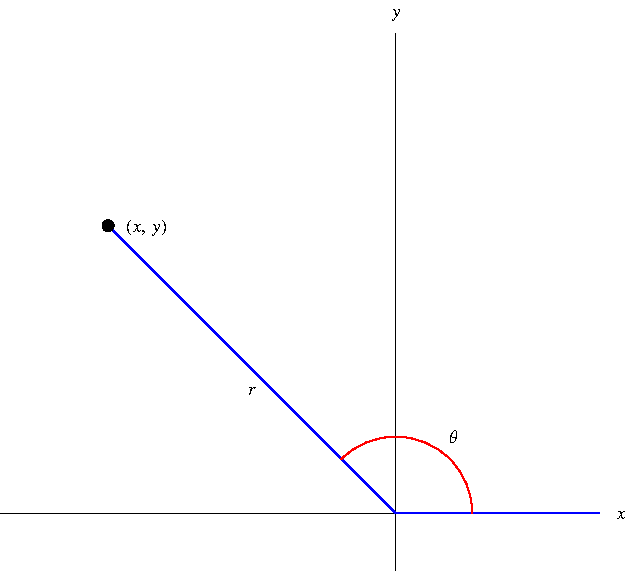
\includegraphics[width=5cm]{trigonometry/pictures/app-d-ratiosb.pdf}%
\[
\begin{array}{cc}
\sin \theta = \frac{ y}{ r} &
\csc \theta = \frac{ r}{ y} \\
\cos \theta = \frac{ x}{ r} &
\sec \theta = \frac{ r}{ x} \\
\tan \theta = \frac{ y}{ x} &
\cot \theta = \frac{ x}{ y} \\
\end{array}
\]
\column{.5\textwidth}
\begin{itemize}
\item $\csc \theta = \frac{1}{\sin \theta}$
\item $\sec \theta = \frac{1}{\cos \theta}$
\item $\cot \theta = \frac{1}{\tan \theta}$
\item $\tan \theta = \frac{\sin \theta}{\cos \theta}$
\item $\cot \theta = \frac{\cos \theta}{\sin \theta}$
\end{itemize}
\end{columns}
\end{frame}


\begin{frame}
\begin{columns}[c]
\column{.5\textwidth}
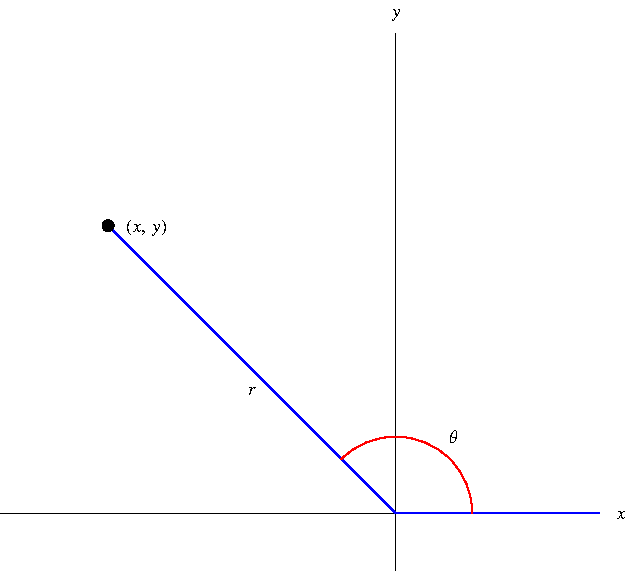
\includegraphics[width=5cm]{trigonometry/pictures/app-d-ratiosb.pdf}%
\[
\begin{array}{cc}
\sin \theta = \frac{ y}{ r} &
\csc \theta = \frac{ r}{ y} \\
\cos \theta = \frac{ x}{ r} &
\sec \theta = \frac{ r}{ x} \\
\tan \theta = \frac{ y}{ x} &
\cot \theta = \frac{ x}{ y} \\
\end{array}
\]
\column{.5\textwidth}
\begin{eqnarray*}
& & \uncover<2->{\sin^2 \theta + \cos^2 \theta}\\
& \uncover<3->{=} & \uncover<3->{\frac{y^2}{r^2} + \frac{x^2}{r^2}}\\
& \uncover<4->{=} & \uncover<4->{\frac{y^2+x^2}{r^2}}\\
& \uncover<5->{=} & \uncover<5->{\frac{r^2}{r^2}}\\
& \uncover<6->{=} & \uncover<6->{1}
\end{eqnarray*}
\uncover<7->{%
Therefore $\sin^2 \theta + \cos^2 \theta = 1$.%
}%
\end{columns}
\end{frame}


\begin{frame}
\begin{columns}[c]
\column{.5\textwidth}
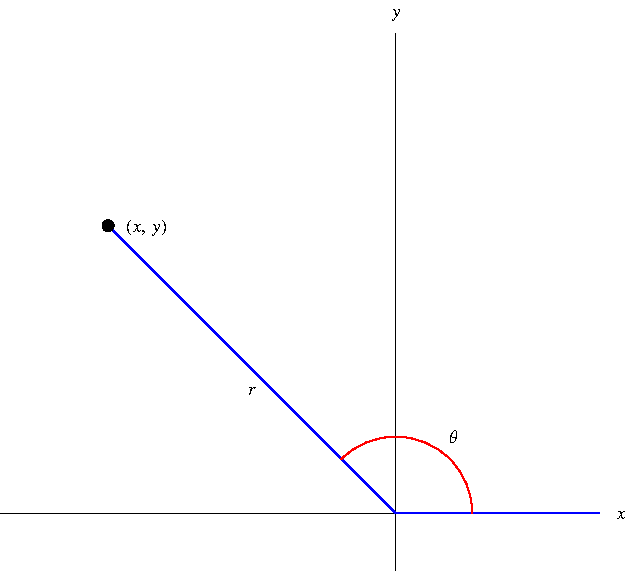
\includegraphics[width=5cm]{trigonometry/pictures/app-d-ratiosb.pdf}%
\[
\begin{array}{cc}
\sin \theta = \frac{ y}{ r} &
\csc \theta = \frac{ r}{ y} \\
\cos \theta = \frac{ x}{ r} &
\sec \theta = \frac{ r}{ x} \\
\tan \theta = \frac{ y}{ x} &
\cot \theta = \frac{ x}{ y} \\
\end{array}
\]
\column{.5\textwidth}
\begin{example}[$\tan^2 \theta + 1 = \sec^2 \theta$]
Prove the identity $\tan^2 \theta + 1 = \sec^2 \theta$.
\begin{eqnarray*}
\uncover<2->{\sin^2 \theta + \cos^2 \theta} & \uncover<2->{=} & \uncover<2->{1}\\
\uncover<3->{\frac{\sin^2 \theta}{\cos^2\theta} + \frac{\cos^2 \theta}{\cos^2\theta}} & \uncover<3->{=} & \uncover<3->{\frac{1}{\cos^2\theta}}\\
\uncover<4->{\tan^2 \theta + 1} & \uncover<4->{=} & \uncover<4->{\sec^2\theta}
\end{eqnarray*}
\end{example}
\end{columns}
\end{frame}



\begin{frame}
\begin{columns}[c]
\column{.5\textwidth}
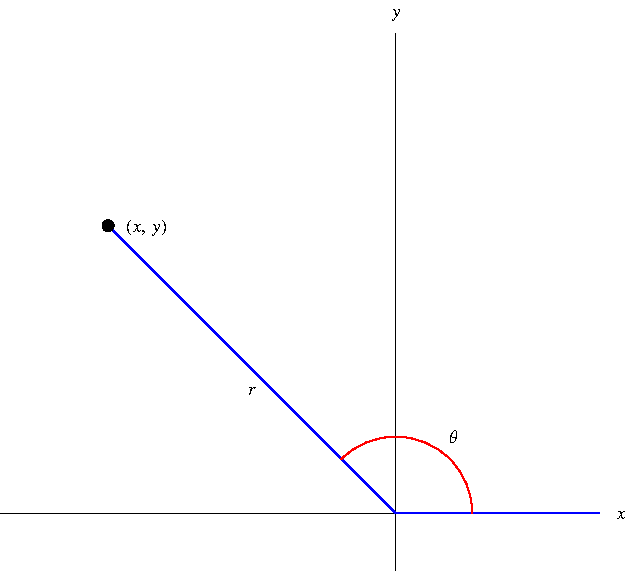
\includegraphics[width=5cm]{trigonometry/pictures/app-d-ratiosb.pdf}%
\[
\begin{array}{cc}
\sin \theta = \frac{ y}{ r} &
\csc \theta = \frac{ r}{ y} \\
\cos \theta = \frac{ x}{ r} &
\sec \theta = \frac{ r}{ x} \\
\tan \theta = \frac{ y}{ x} &
\cot \theta = \frac{ x}{ y} \\
\end{array}
\]
\column{.5\textwidth}
\begin{itemize}
\item<2->  Positive angles are obtained by rotating counterclockwise.
\item<2->  Negative angles are obtained by rotating clockwise.
\item<3->  If $(x,y)$ is on the terminal arm of the angle $\theta$, then $(x, -y)$ is on the terminal arm of $-\theta$.
\item<4->  $\sin(-\theta ) = \frac{-y}{r} = -\frac{y}{r} = -\sin \theta$.
\item<5->  $\cos(-\theta ) = \frac{x}{r} = \cos \theta$.
\item<6->  $\sin$ is an odd function.
\item<7->  $\cos$ is an even function.
\end{itemize}
\end{columns}
\end{frame}



\begin{frame}
\begin{columns}[c]
\column{.5\textwidth}
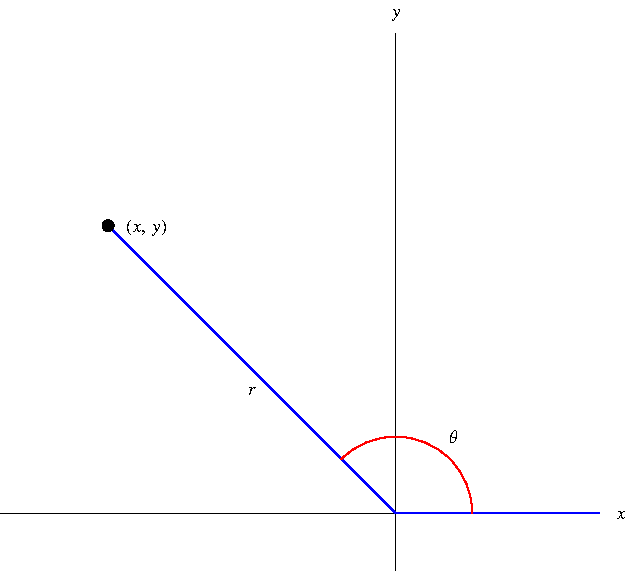
\includegraphics[width=5cm]{trigonometry/pictures/app-d-ratiosb.pdf}%
\[
\begin{array}{cc}
\sin \theta = \frac{ y}{ r} &
\csc \theta = \frac{ r}{ y} \\
\cos \theta = \frac{ x}{ r} &
\sec \theta = \frac{ r}{ x} \\
\tan \theta = \frac{ y}{ x} &
\cot \theta = \frac{ x}{ y} \\
\end{array}
\]
\column{.5\textwidth}
\begin{itemize}
\item<2->  $2\pi$ represents a full rotation.
\item<3->  $\theta + 2\pi$ has the same terminal arm as $\theta$.
\item<4->  $\theta + 2\pi$ uses the same point $(x,y)$ and the same length $r$.
\item<5->  $\sin (\theta + 2\pi ) = \sin \theta$.
\item<5->  $\cos (\theta + 2\pi ) = \cos \theta$.
\item<6->  We say $\sin$ and $\cos$ are $2\pi$-periodic.
\end{itemize}
\end{columns}
\end{frame}


\begin{frame}[t]
The remaining identities are consequences of the addition formulas:
\[
\begin{array}{ccccc}
\sin (x + y) & = & \sin x\cos y & + & \cos x \sin y \\
\cos (x + y) & = & \cos x\cos y & - & \sin x \sin y 
\end{array}
\]
\uncover<2->{
Substitute $-y$ for $y$, and use the fact that $\sin(-y) = -\sin y$ and $\cos (-y) = \cos y$:
\[
\begin{array}{ccccc}
\sin (x - y) & = & \sin x\cos y & - & \cos x \sin y \\
\cos (x - y) & = & \cos x\cos y & + & \sin x \sin y 
\end{array}
\]
}
\end{frame}


\begin{frame}[t]
The remaining identities are consequences of the addition formulas:
\[
\begin{array}{ccccc}
\sin (x + y) & = & \sin x\cos y & + & \cos x \sin y \\
\cos (x + y) & = & \cos x\cos y & - & \sin x \sin y 
\end{array}
\]
\uncover<2->{
To get the double angle formulas, substitute $x$ for $y$:
\[
\begin{array}{rcl}
\sin 2x  & = & 2\sin x\cos x \\
\cos 2x  & = & \cos^2 x - \sin^2 x
\end{array}
\]
}
\uncover<3->{
Rewrite the second double angle formula in two ways, using $\cos^2 x = 1 - \sin^2 x$ and $\sin^2 x = 1 - \cos^2 x$:
\[
\begin{array}{rcl}
\cos 2x  & = & 2\cos^2 x  -1\\
\cos 2x  & = & 1 - 2\sin^2 x
\end{array}
\]
}
\uncover<4->{
To get the half-angle formulas, solve these equations for $\cos^2 x$ and $\sin^2 x$ respectively.
\[
\cos^2 x = \frac{1 + \cos 2x}{2}, \qquad \sin^2 x = \frac{1 - \cos 2x}{2} 
\]
}
\end{frame}


\begin{frame}[t]
The remaining identities are consequences of the addition formulas:
\[
\begin{array}{ccccc}
\sin (x + y) & = & \sin x\cos y & + & \cos x \sin y \\
\cos (x + y) & = & \cos x\cos y & - & \sin x \sin y 
\end{array}
\]
\uncover<2->{
Divide the first equation by the second, and then cancel $\cos x \cos y$ from the top and bottom:
\[
\begin{array}{rcl}
\tan (x + y)  & = & \frac{\tan x + \tan y}{1 - \tan x \tan y}
\end{array}
\]
}
\uncover<3->{
Do the same for the subtraction formulas:
\[
\begin{array}{rcl}
\tan (x - y)  & = & \frac{\tan x - \tan y}{1 + \tan x \tan y}
\end{array}
\]
}
\end{frame}
% end module trig-identities
